\documentclass[en]{snu-cse-bsc-thesis}

% Add your packages here, e.g.,
% \usepackage{tikz}
\usepackage{siunitx}

% For lorem ipsum; remove these lines when writing your thesis
\usepackage{lipsum}
\usepackage{jiwonlipsum}

% hyperref *must* be the last package to be loaded!
\usepackage[pdfusetitle]{hyperref}
\usepackage{indentfirst}

\addbibresource{bib.bib}

\title{Two Layer Path Planning for Multi-Map Navigation}
\titlealt{다중 지도 네비게이션을 위한 이중 레이어 경로 계획}
\author{장준서}
\advisor{홍길동}
\date{2025년 월 일}
\approvaldate{2025년 8월}

\koreankeywords{경로 계획, 자율 이동 로봇, 다중 지도 네비게이}
\englishkeywords{Path Planning, Autonomous Mobile Robot, Multi Map Navigation}


\begin{document}
\maketitle

\pagenumbering{roman}
\begin{abstract}
This paper presents a hierarchical path-planning approach designed for robots operating across multiple maps. The proposed method utilizes a hybrid map structure consisting of two layers: an upper-layer graph that represents navigational waypoints and transitions between maps, and a lower-layer occupancy grid that provides detailed spatial information for precise movement.  

Path planning is performed in three stages. First, the robot's current position is added as a node to the upper-layer graph. Second, a high-level path is computed using a shortest-path algorithm to determine the waypoints the robot must pass through. Finally, the lower layer is used to generate a detailed navigation path between waypoints while dynamically considering real-time positioning and obstacles.  

This approach enables seamless navigation in large spaces, including multi-story buildings, by effectively managing map transitions through designated horizontal map change points and elevator nodes. The method ensures scalability and flexibility, allowing robots to operate efficiently across extensive areas. Future work will explore automatic generation of upper-layer nodes and real-time updates to further enhance adaptability.

\end{abstract}

\tableofcontents
\listoftables
\listoffigures

\chapter{Introduction}\label{chap:introduction}
\pagenumbering{arabic}
With advancements in autonomous driving technology, various autonomous robots are being utilized in everyday life. Representative examples include service robots that shuttle between kitchens and tables to deliver food and utensils~\cite{ServiPlus}, cleaning robots that roam specific areas to perform cleaning and disinfection tasks~\cite{ServiAir}, and logistics robots that transport goods in large warehouses~\cite{Carti100}.

These robots typically operate within designated areas, performing simple, repetitive tasks. As the demand for autonomous robots continues to grow, the size of the areas each robot must manage has also expanded. Whereas traditional service robots were confined to operating within the boundaries of a small restaurant, they are now required to transport food or goods across large shopping malls with multiple restaurants or multi-story office buildings~\cite{ServiLift}.

The expansion of operational areas has introduced several technical challenges. One such challenge is the inability to cover all areas using a single map. Autonomous robots rely on pre-constructed maps to determine their current location and calculate routes to their destinations. However, if a large operational area is represented using a single map, the computational load becomes excessively high, leading to inefficiency. A solution to this problem is dividing the operational area into multiple maps. This approach reduces the size of each map, enabling more efficient localization and easier maintenance. 

However, when the starting point and destination are located on different maps, conventional path-planning methods such as A* or RRT cannot compute a path. These methods operate under the assumption that both points lie within the same map. Therefore, a path-planning algorithm for new data structure, multiple maps, is necessary. The paper ~\cite{MultiStoreyBuildingNavigation} proposes a path-planning method for navigating between different floors of multi-storey buildings. In this study, the robot's operational area is represented as a hybrid map composed of multiple layers. The upper layer contains topological information, such as the building and floor details of specific locations, while the lower layer holds metric information, such as an occupancy grid map. Using this hybrid map, the robot performs hierarchical path planning to identify the waypoints required for navigation.

This report builds upon the aforementioned study and explains the implementation of a path-planning method for navigating between arbitrary start and destination points across multiple maps—a task the author undertook at Bear Robotics. The path-planning process consists of two main stages: 1) High-level path planning, which operates on a graph composed of nodes that connect different maps. This stage determines which maps to traverse and which nodes to pass through to move from the starting point to the destination. 2) Low-level path planning, which calculates the global path within a single map to travel between nodes. By combining high-level and low-level path planning, the method ensures efficient navigation across multiple maps while managing the complexity of larger operational areas.

The remainder of this report is organized as follows:
Chapter 2 explains the background knowledge for autonomous robot navigation; Chapter 3 details the data structure to represent operational areas and path planning method across multiple maps; and Chapter 4 concludes the report.

% This template is structured as follows.
% Section~\ref{sec:figure} of chapter~\ref{chap:body} shows an example of a figure.
% Section~\ref{sec:table} of chapter~\ref{chap:body} shows an example of a table.
% Chapter~\ref{chap:conclusion} concludes this template.

% \section{Section Sample}\label{sec:section}
% \lipsum[2-3]


\chapter{Body}\label{chap:body}

\section{Methodology}\label{sec:Methodology}
The implemented path-planning method operates on a hybrid map consisting of two layers. The lower layer consists of occupancy grid maps, each uniquely identified by an ID and possessing its own independent coordinate system. During navigation, the robot uses a map corresponding to the current location, and its position is expressed in the coordinate system of that specific map. When a horizontal area is too large and must be divided into multiple maps, overlapping regions are introduced between adjacent maps. These common regions ensure seamless localization when the robot transitions from one map to another, allowing for accurate position estimation even after switching maps.

The upper layer is a graph, where nodes are categorized into three types:
\begin{enumerate}
  \item Destination: Represents final destinations such as tables in a restaurant or storage locations in a warehouse.
  \item Horizontal Map Change Point: Represents transition points between different maps on the same floor. These points exist within the overlapping regions of two maps and are conceptually identical locations but have separate nodes for each map. Multiple points can connect two specific maps, and a single point may connect three or more maps.
  \item Elevator: Represents the location of a specific elevator on a given floor. Although an elevator may serve multiple floors, a separate node is defined for each floor's boarding point.
\end{enumerate}
Each node contains various information such as location coordinates, floor number and the map ID to which it belongs, and the connected map IDs.

To make a graph, nodes should be connected by edges. The conditions for creating edges between nodes are as follows:
\begin{enumerate}
  \item Within the same map: Nodes on the same map are connected. The edge weight between two nodes is determined by the path's length between them. The path is calculated using an occupancy grid map in the lower layer and traditional path planning method, like A*.
  \item Between horizontal map change points: Nodes representing the same location across different maps are connected. As the actual distance between the two nodes is 0, the edge weight between such nodes is set to 0.
  \item Between elevator nodes: Nodes representing the same elevator across different floors are connected. As the robot won't move while elevator is moving, the edge weight between these nodes is also set to 0.
\end{enumerate}
An example of this graph structure can be seen in Figure ~\ref{fig:graph_outline}.
\begin{figure}[!t]
  \centering
  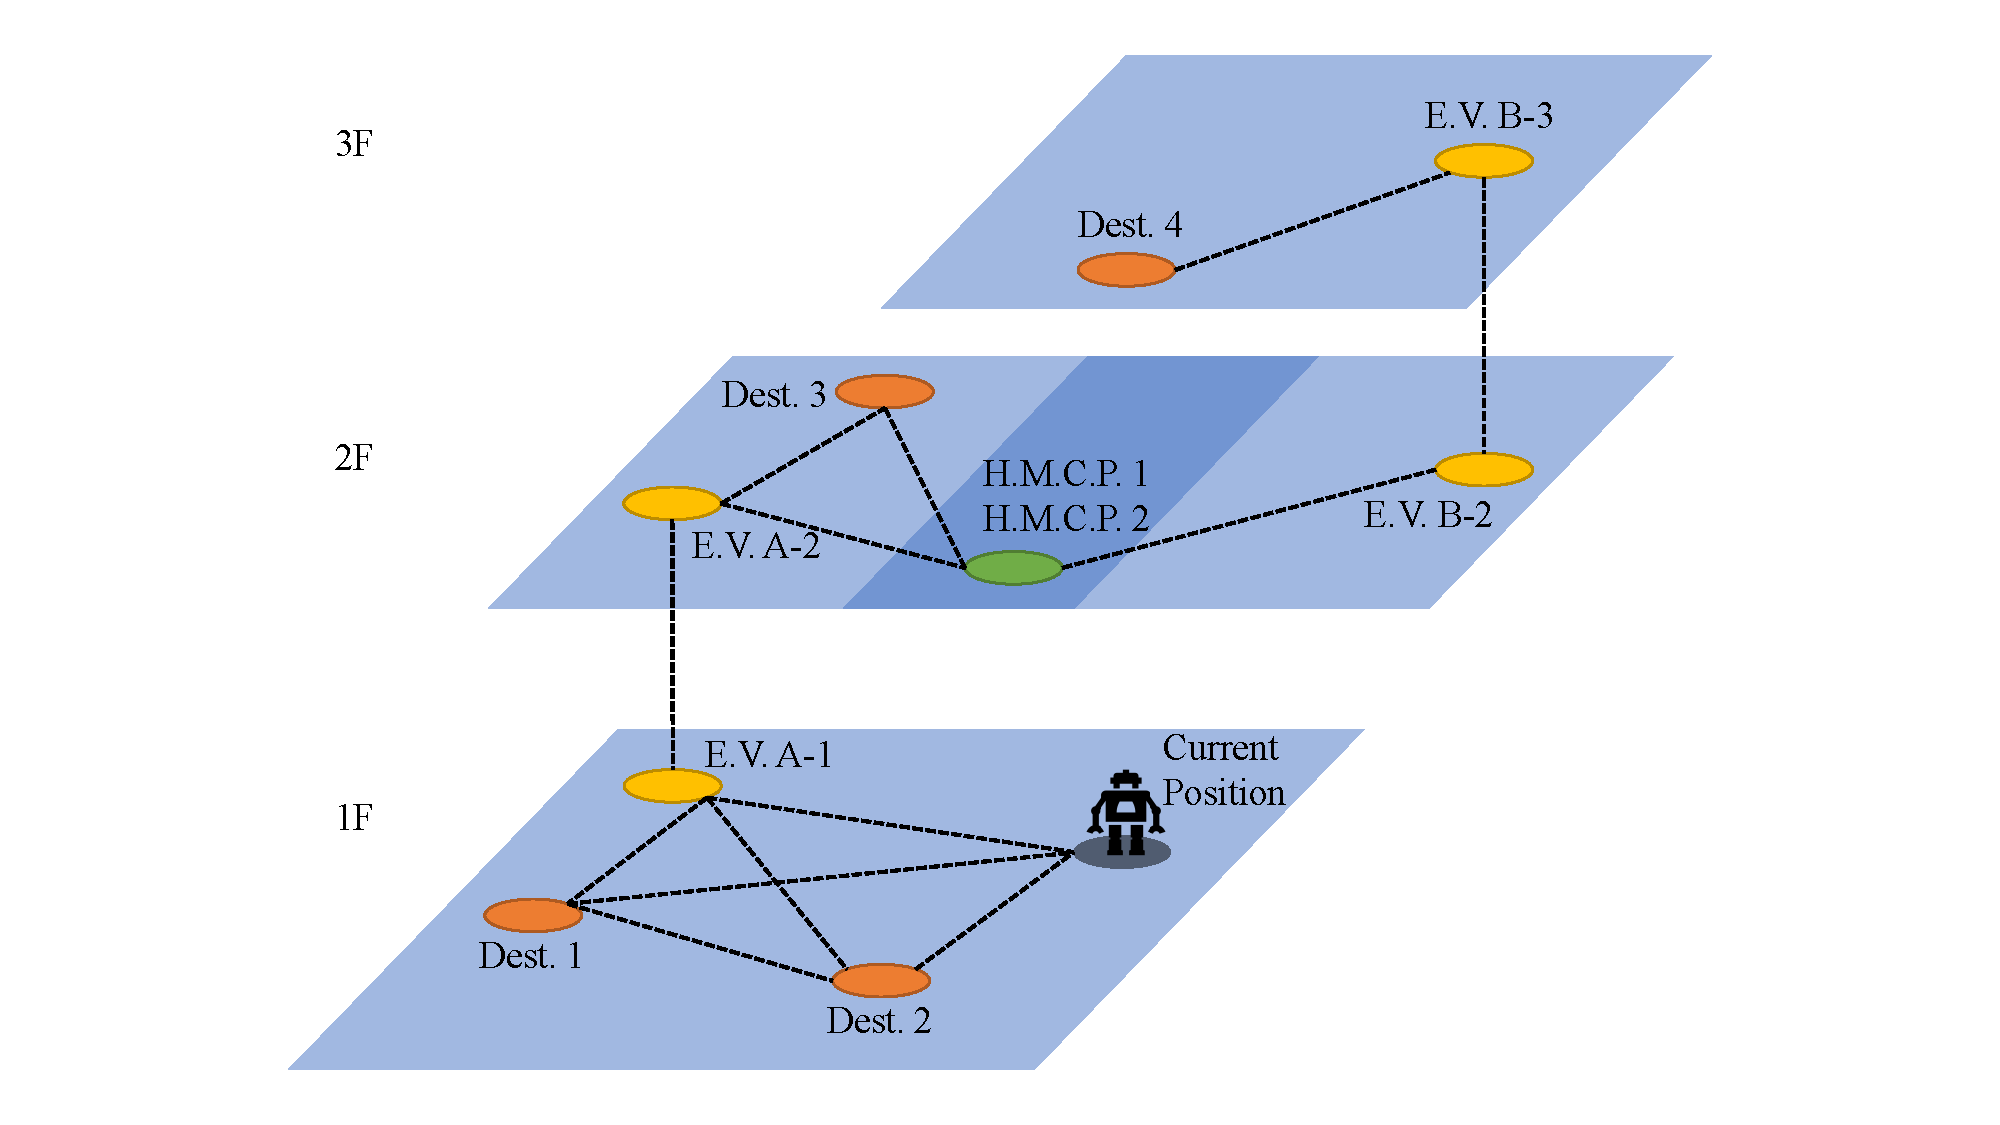
\includegraphics[width=0.8\textwidth]{gcg graph outline.pdf}
  \caption{This figure illustrates an example of the upper layer of a hybrid map for a three-story building. The building is structured such that the 1st and 2nd floors are connected by Elevator A, while the 2nd and 3rd floors are connected by Elevator B. On the 1st floor, where the robot is currently located, the map includes two destination nodes and one elevator node representing Elevator A. The black node represents the robot's current location. Since it is a temporary node, it will be removed when the path planning is finished. The 2nd floor is divided into two separate maps: the left map contains one destination node, one elevator node for Elevator A, and one horizontal map change point (H.M.C.P. 1) that connects the left and right maps. The right map includes one elevator node for Elevator B and one horizontal map change point (H.M.C.P. 2) that connects the two maps on this floor. Although H.M.C.P. 1 and H.M.C.P. 2 are defined in the coordinate systems of their respective maps, they represent the same physical location. On the 3rd floor, the map includes one elevator node for Elevator B and one destination node.}
  \label{fig:graph_outline}
\end{figure}

Path planning consists of three main stages. The first stage involves adding the current position as a new node of type "destination" to the upper-layer graph. Following the edge creation rules described earlier, edges are then connected between this new node and other nodes within the same map. If the starting point is not the current position but an existing node, this step is skipped.

The second stage calculates the shortest path from the starting node to the destination node in the upper layer. A single-source, single-destination shortest path algorithm, such as Dijkstra’s algorithm, is used for this purpose. This stage determines the waypoints the robot must pass through to reach its destination. Importantly, this step is performed only once, before the robot begins its journey.

The third stage involves performing global path planning in the lower layer to navigate from the current position to the next waypoint. This stage is similar to navigation within a single map, where real-time information such as the robot's current position and obstacles is used to compute the global path and local path. This process continues until the robot reaches the final destination.

\section{Example of Implementation}\label{sec:Example}
An example is illustrated in Figure ~\ref{fig:graph_outline}. Suppose the destinations are given as Dest. 4, Dest. 3, Dest. 2, and Dest. 1. First, the robot's current position is added to the graph, as shown in the figure. Then, Dijkstra’s algorithm is used to calculate the shortest path from the current position to Dest. 4. The resulting node array is “E.V A-1, E.V A-2, H.M.C.P 1, H.M.C.P. 2, E.V B-2, E.V B-3, Dest. 4”. The process is repeated by updating the starting point to the current destination and calculating the shortest path to the next destination. The results of these calculations can be found in Table ~\ref{tab: high level path planning}.

After high-level path planning is completed, low-level path planning is performed. Figure ~\ref{fig:first_floor_low_level_pp} illustrates the robot performing path planning to reach the first waypoint, E.V A-1. Low-level path planning continues iteratively until no waypoints remain.

\section{Discussion}\label{sec:Discussion}
Unlike ~\cite{MultiStoreyBuildingNavigation}, this path-planning method uses only two layers. Earlier research structured nodes into multiple levels, such as building, floor, and region. In contrast, this implementation uses a single semantic layer, where each node contains all necessary information, including building ID, floor number, and map ID. The reason for not using multiple levels is to improve scalability. As the number of properties such as floor and region increases, distinguishing their hierarchical levels will become more challenging and the topological graph will become harder to manage. To avoid this complexity, all semantic nodes are placed at the same level, and the relationships between them are handled through edge connections. This approach makes the system more flexible and easier to expand.

This method allows for easy integration with other elements using waypoints. The robot's screen can display the current waypoint as the destination, making it intuitive for users to understand the robot's movements. Additionally, specific actions to reach a given waypoint can be easily created using finite state machines (FSM) or behavior trees. For example, if the next two waypoints are elevators on the first floor and the second floor, a behavior tree could be structured as follows: "Move", "Board Elevator", "Press 2nd Floor Button" → "Wait" → "Exit Elevator".

However, there are drawbacks. One major issue is that it takes a long time to create the upper layer in advance. Horizontal map change points and elevators must be manually specified. Moreover, since all nodes within the same map must be interconnected, the graph size increases significantly as the number of nodes increases. As the number and types of nodes increase, system maintenance will become more difficult. Additionally, if the starting point is the robot's current position, robot needs a time to add a new node to the graph. Longer loading times between setting the destination and moving can lead to a bad user experience. Therefore, it is important to divide the space using a reasonable number of maps, ensuring that there are not too many nodes within a single map while still avoiding excessive maps overall.

\begin{table}[!b]
  \centering
  \caption[Table example (ToC)]{Results of high-level path planning of given destinations.}\label{tab: high level path planning}
  \begin{tblr}{llp{10cm}}
    \toprule
    Start Node & End Node & Waypoints \\\midrule
    "Current Position" & "Dest. 4" & 
      "E.V. A-1", "E.V. A-2", "H.M.C.P. 1", "H.M.C.P. 2", \newline "E.V. B-2", "E.V. B-3", "Dest. 4"
     \\

    "Dest. 4" & "Dest. 3" & 
      "E.V. B-3", "E.V. B-2", "H.M.C.P. 2", "H.M.C.P 1", "Dest. 3"
     \\
    
    "Dest. 3" & "Dest. 2" & 
      "E.V. A-2", "E.V. A-1", "Dest. 2"
     \\
    
    "Dest. 2" & "Dest. 1" & 
      "Dest. 1"
     \\
    \bottomrule
  \end{tblr}
\end{table}

\begin{figure}[!t]
  \centering
  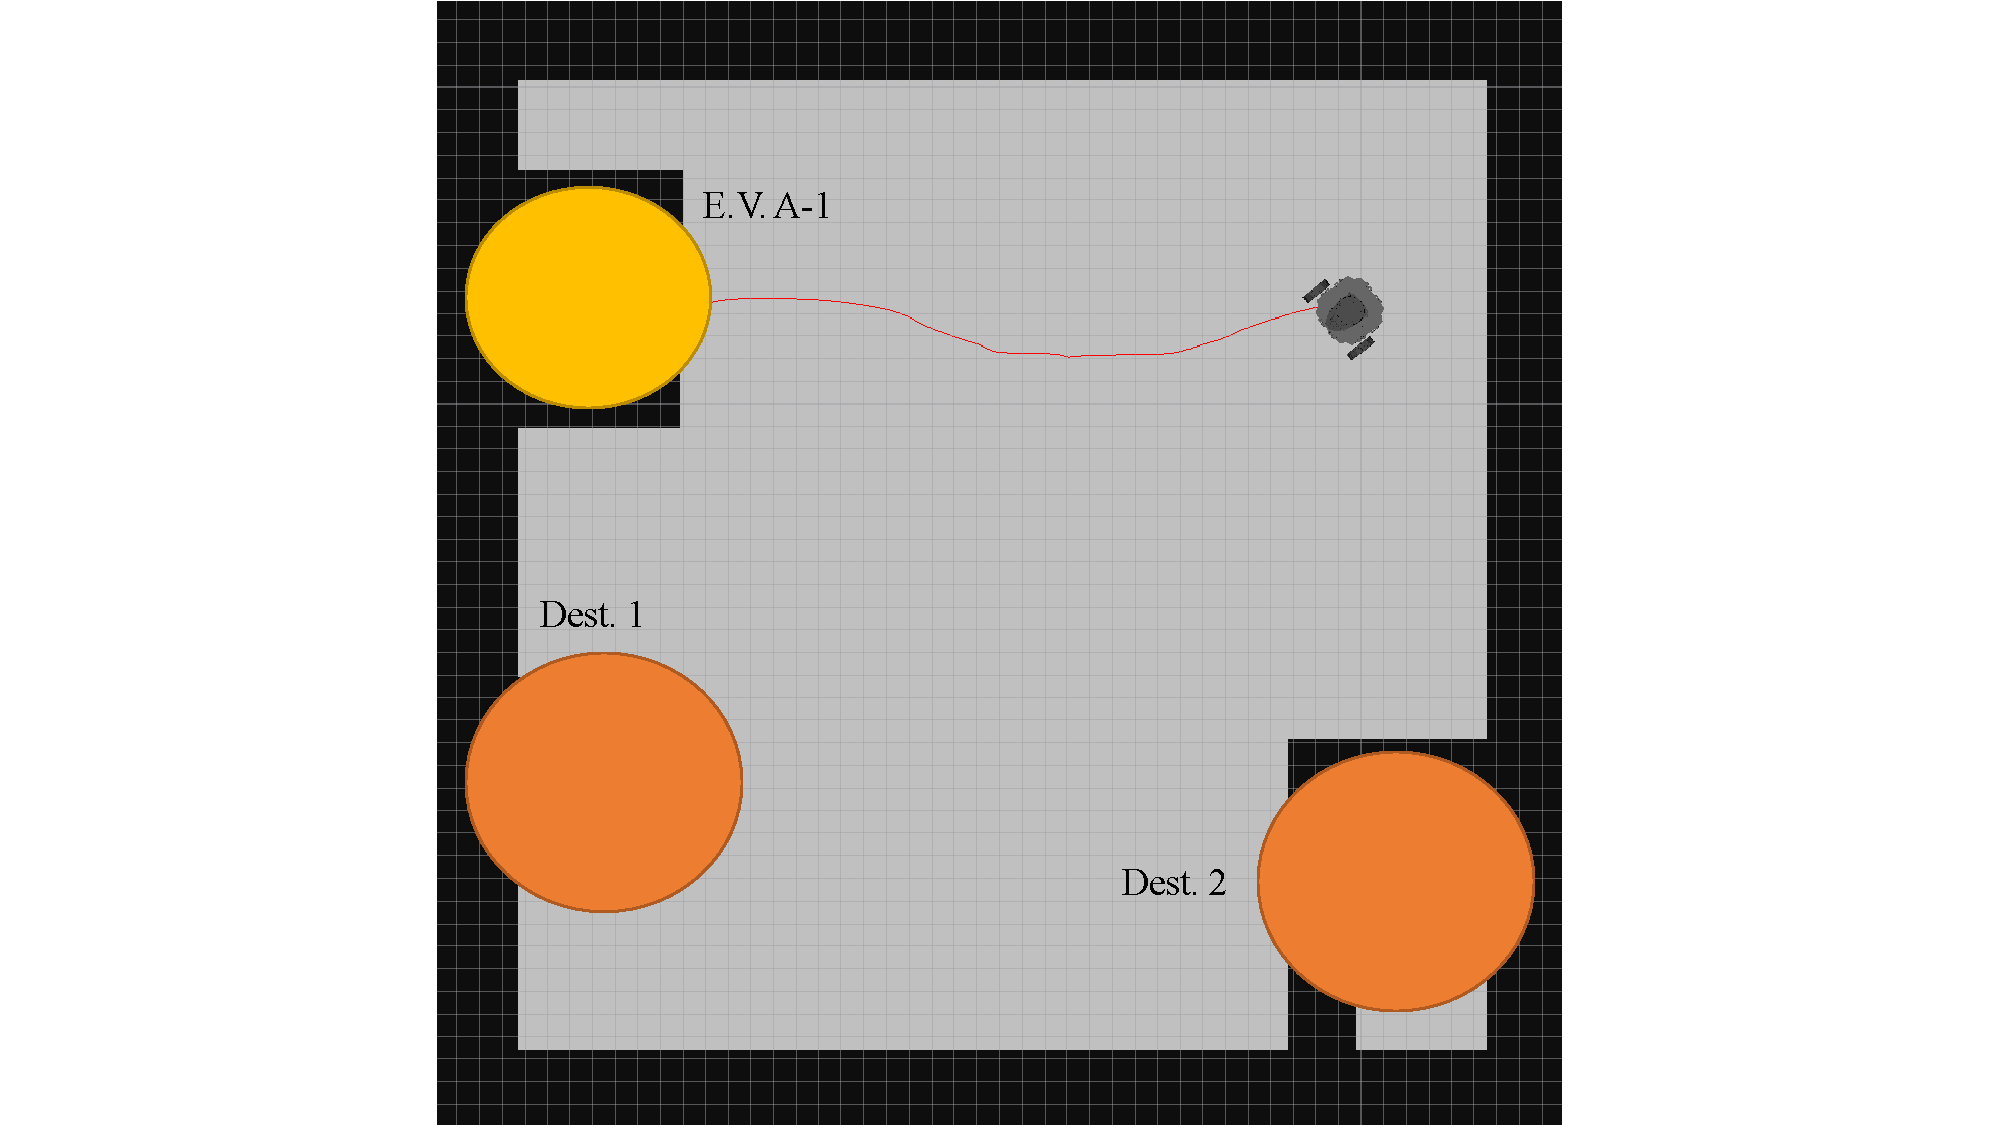
\includegraphics[width=0.8\textwidth]{first_floor_low_level_pp.pdf}
  \caption{Example of low-level path planning from "Current Position" to the first waypoint, "E.V. A-1".}
  \label{fig:first_floor_low_level_pp}
\end{figure}

% Entropy of information is the expected value of information contained in each message, and is given by equation~\eqref{eq:entropy}~\cite{6773024}.
% \begin{equation}\label{eq:entropy}
%   H(X) = -\sum_{i=1}^n {\mathrm{P}(x_i) \log_b \mathrm{P}(x_i)}
% \end{equation}

% \lipsum[4-6]


% \section{Figure}\label{sec:figure}
% Example of a figure is shown in figure~\ref{fig:example}.
% Figure~\ref{fig:snu} is the logo of Seoul National University and figure~\ref{fig:eng} is the logo of College of Engineering.

% \begin{figure}[!t]
%   \centering
%   \begin{subfigure}[b]{0.5\textwidth}
%     \centering
%     
\includegraphics[width=0.5\textwidth]{logo1.pdf}
%     \caption{The logo of Seoul National University}\label{fig:snu}
%   \end{subfigure}%
%   \begin{subfigure}[b]{0.5\textwidth}
%     \centering
%     
\includegraphics[width=0.9\textwidth]{logo2.pdf}
%     \caption{The logo of College of Engineering}\label{fig:eng}
%   \end{subfigure}
%   \caption[Figure example (ToC)]{An example of a figure.}\label{fig:example}
% \end{figure}

% \lipsum[7-8]


% \section{Table}\label{sec:table}
% Example of a table is shown in table~\ref{tab:example}.\footnote{\lipsum[12]}

% \begin{table}[htp]
%   \centering
%   \caption[Table example (ToC)]{An example of a table.}\label{tab:example}
%   \begin{tblr}{cc}
%     \toprule
%     Constant & Value \\\midrule
%     $c$ & \SI{299792458}{\meter\per\second} \\
%     $h$ & \SI{6.62607015e-34}{\joule\per\hertz} \\\bottomrule
%   \end{tblr}
% \end{table}

% \lipsum[9-10]


\chapter{Conclusion}\label{chap:conclusion}
This report explains the path-planning method I implemented at Bear Robotics. It used in situations requiring multiple maps, like a multi-floor building. The proposed approach utilizes a new map structure consisting of two layers. By performing hierarchical path planning within each layer, the system can calculate routes between different locations. High level path planning provides a waypoint, such as the elevator, needed to move to another map. Low level path planning provides path or trajectory using conventional methodologies such as A* or RRT. This method allows robots to navigate freely across large spaces and accurately reach their destinations, even in multi-story buildings. In addition, the waypoints from high level path planning can clearly express the robot's path to users. In the future, this approach could be further improved by automating the generation of upper-layer nodes or dynamically updating the upper layer with real-time position data.

\printbibliography

\begin{abstract}[ko]
본 보고서에서는 여러 개의 지도를 활용하는 로봇을 위한 계층적 경로 계획 기법을 제안한다. 제안된 방법은 두 개의 layer로 구성된 하이브리드 맵 구조를 사용한다. 상위 layer는 그래프 구조로, 지도 간의 전환과 주요 경유지를 나타내며, 하위 layer는 점유 그리드 맵을 활용하여 정밀한 이동을 가능하게 한다.  

경로 계획은 세 단계로 이루어진다. 첫째, 로봇의 현재 위치를 상위 layer의 그래프에 새로운 노드로 추가한다. 둘째, 최단 경로 알고리즘을 사용하여 로봇이 거쳐야 할 waypoint를 계산한다. 셋째, 하위 layer에서 실시간 위치 및 장애물 정보를 고려하여 waypoint 간의 세부 이동 경로를 생성한다.  

이 방법은 수평 지도 전환 지점(Horizontal Map Change Point)과 엘리베이터 노드를 활용하여 넓은 공간 및 다층 건물에서도 원활한 이동을 가능하게 한다. 또한 확장성과 유연성을 보장하여 로봇이 광범위한 환경에서도 효과적으로 작동할 수 있도록 한다. 향후 연구에서는 상위 layer의 노드를 자동으로 생성하거나 실시간으로 업데이트하는 방식을 도입하여 적응성을 더욱 향상할 예정이다.

\end{abstract}
\end{document}
